\documentclass[10pt,letterpaper]{article}
%----------------------------------------------------------------------------------------
%	PACKAGES AND OTHER DOCUMENT CONFIGURATIONS
%----------------------------------------------------------------------------------------

\usepackage{amsmath,amsfonts,stmaryrd,amssymb} % Math packages
\usepackage{amsfonts}
\usepackage{float}
\usepackage{enumerate} % Custom item numbers for enumerations
\usepackage{mathtools}
\usepackage{mathrsfs}
\usepackage{commath}
\usepackage[ruled]{algorithm2e} % Algorithms
\newtheorem{proof}{PROOF}
\usepackage[framemethod=tikz]{mdframed} % Allows defining custom boxed/framed environments

\usepackage[T1]{fontenc}
\usepackage{bigfoot} % to allow verbatim in footnote
\usepackage{python}
\usepackage{graphicx}
\usepackage{geometry}
% \userpackage{pdfpages}

\usepackage{lipsum}


\newcommand{\overbar}[1]{\mkern 1.5mu\overline{\mkern-1.5mu#1\mkern-1.5mu}\mkern 1.5mu}
\geometry{letterpaper, portrait, margin=1.5cm}

\title{ECE421 Introduction to Machine Learning \\
    Assignment \#2 \\
    Neural Networks}
\date{Feb 2019}
\author{
  Yan, Xuanming\\
  \texttt{xuanming.yan@mail.utoronto.ca} \\
  1001175382 \\
  Contribution: 50\%
  \and
  Wang, Chu Qing\\
  \texttt{eliza.wang@mail.utoronto.ca} \\
  1001303573\\
  Contribution: 50\%
} % Author name and email address
\usepackage[utf8]{inputenc}
 
\usepackage{listings}
\usepackage{color}
 
\definecolor{codegreen}{rgb}{0,0.6,0}
\definecolor{codegray}{rgb}{0.5,0.5,0.5}
\definecolor{codepurple}{rgb}{0.58,0,0.82}
\definecolor{backcolour}{rgb}{0.95,0.95,0.92}
 
\lstdefinestyle{mystyle}{
    backgroundcolor=\color{backcolour},   
    commentstyle=\color{codegreen},
    keywordstyle=\color{magenta},
    numberstyle=\tiny\color{codegray},
    stringstyle=\color{codepurple},
    basicstyle=\footnotesize,
    breakatwhitespace=false,         
    breaklines=true,                 
    captionpos=b,                    
    keepspaces=true,                 
    numbers=left,                    
    numbersep=5pt,                  
    showspaces=false,                
    showstringspaces=false,
    showtabs=false,                  
    tabsize=2
}
 
\lstset{style=mystyle}



\begin{document}
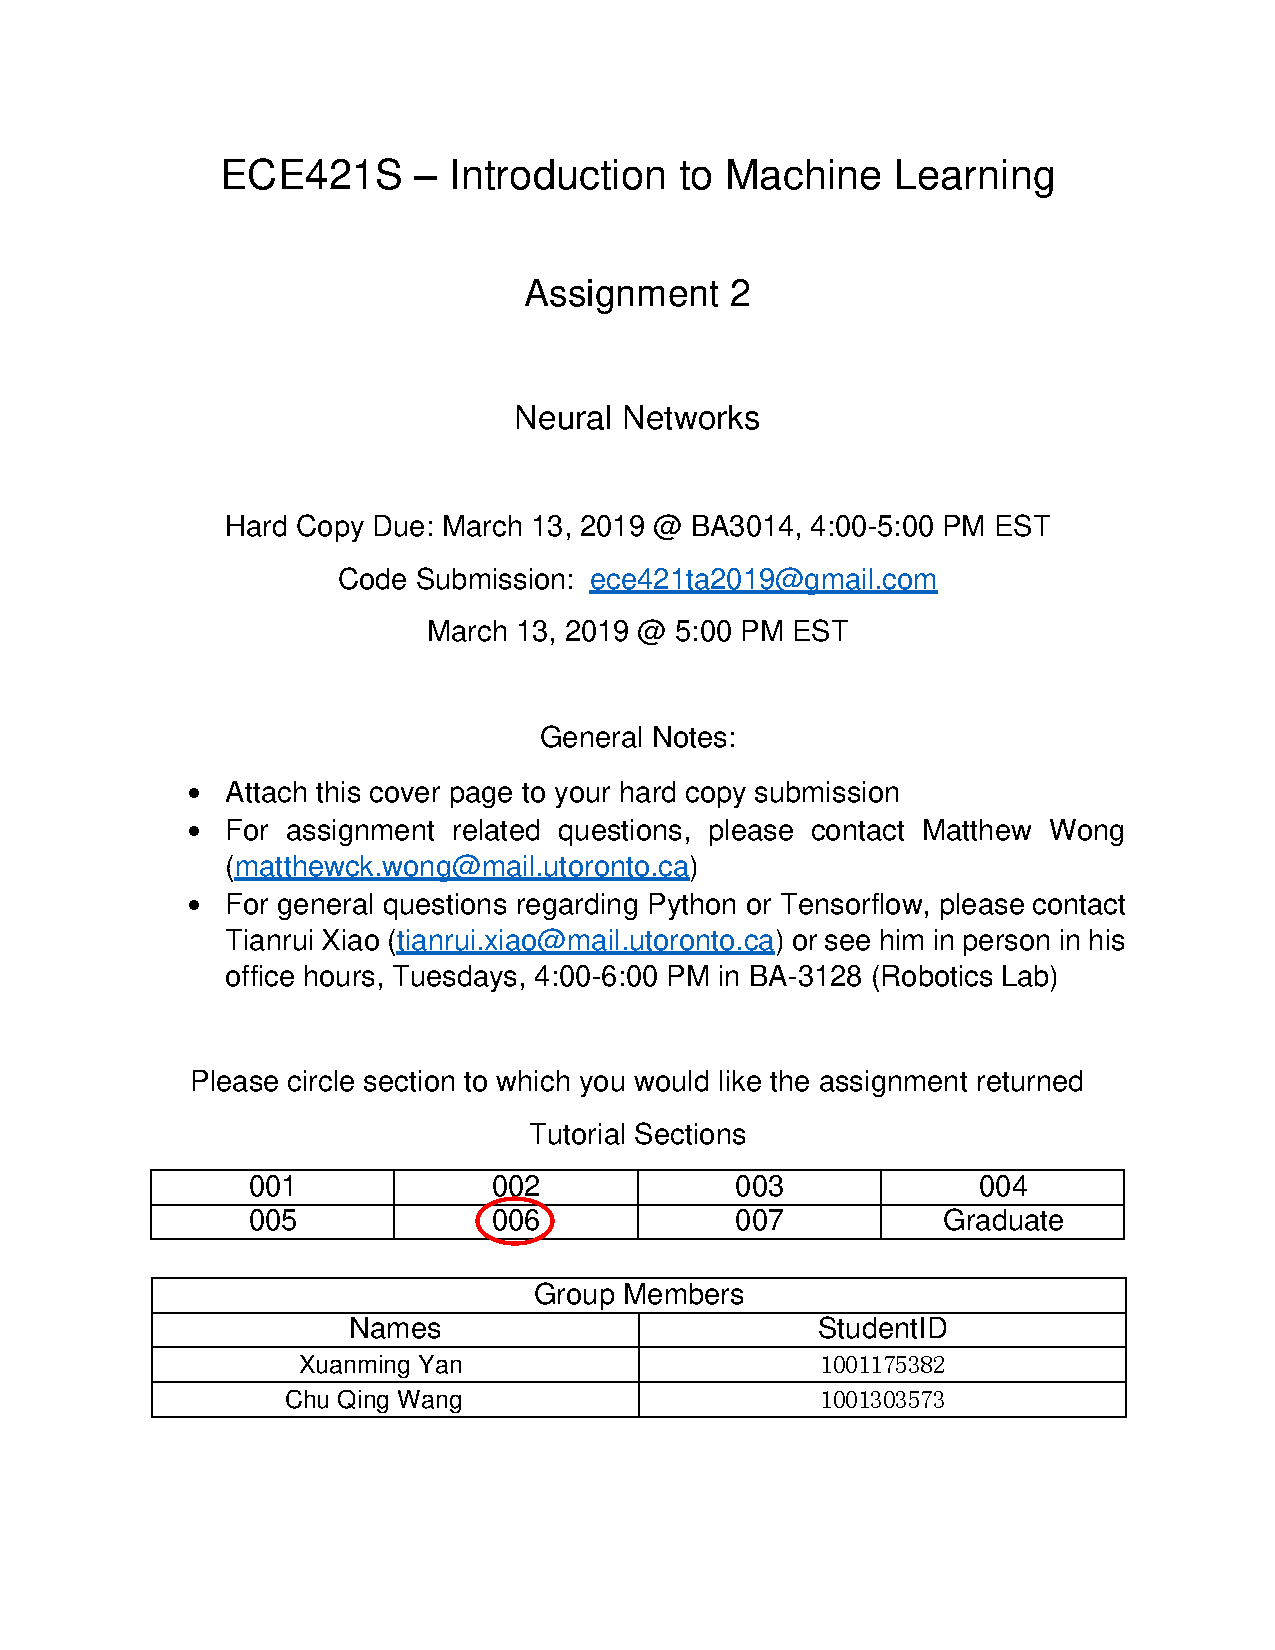
\includegraphics[width=1\linewidth]{a2cover.pdf}


\maketitle % Print the title


\section{Neural Networks using Numpy}


\subsection{Helper Functions}

\begin{enumerate}
  \item \textit{ReLU()}: $ReLU(x) = max(x, 0)$
  \lstinputlisting[language=python, caption = ReLU()]{functions/ReLU.py}
  \item \textit{softmax()}: $\sigma(\textbf{z})_{j} = \frac{e^{z_{j}}}{\sum_{k=1}^{K}e^{z_{k}}}, j = 1\dots K$, for K classes.
  \lstinputlisting[language=python, caption = softmax()]{functions/softmax.py}
   \item \textit{compute()}: 
  \lstinputlisting[language=python, caption = compute()]{functions/compute.py}
   \item \textit{averageCE()}: $CE = -\frac{1}{N}\sum _{k=1}^{K}t_k log(s_k)$
  \lstinputlisting[language=python, caption = averageCE()]{functions/averageCE.py}
   \item \textit{gradCE()}: $ \textbf{z} = \textbf{W}\textbf{x} + \textbf{b}$, $\textbf{s} = softmax(\textbf{z}) = \frac{e^{\textbf{z}}}{\sum_{k=1}^{K}e^{z_{k}}}$, 
   \begin{align*}
        \mathcal{L}_{CE} &= -\sum _{k=1}^{K}t_k log(s_k)\\ &=-\textbf{t}^{T}(log(\textbf{s})) \\
        \frac{\partial \mathcal{L}_{CE}}{\partial  \textbf{s}} &= -\textbf{t}^{T}(\frac{\partial }{\partial  \textbf{s}}(log(\textbf{s})))\\ &= -\textbf{t}^{T}\frac{1}{\textbf{s}}\\
   \end{align*}
   Derivative of softmax can be derived:
   \begin{align*}
       \frac{\partial \textbf{s}}{\partial  \textbf{z}} &= \frac{e^{\textbf{z}}(\sum_{k=1}^{K}e^{z_{k}}) -(e^{\textbf{z}})^{T}e^{\textbf{z}}}{(\sum_{k=1}^{K}e^{z_{k}})^2} \\
       &= \frac{e^{\textbf{z}}}{\sum_{k=1}^{K}e^{z_{k}}}\frac{\sum_{k=1}^{K}e^{z_{k}} - e^{\textbf{z}} }{\sum_{k=1}^{K}e^{z_{k}}} \\
       &= \textbf{s}(1-\textbf{s})
   \end{align*}
   Apply chain rule, we can get: 
   \begin{align*}
              \frac{\partial \mathcal{L}_{CE}}{\partial  \textbf{z}} &=  \frac{\partial \mathcal{L}_{CE}}{\partial  \textbf{s}} \frac{\partial \textbf{s}}{\partial  \textbf{z}}\\ &=(-\textbf{t}^{T}\frac{1}{\textbf{s}})(\textbf{s}(1-\textbf{s}))\\ &= \textbf{s} - \textbf{t}
   \end{align*}
   
  \lstinputlisting[language=python, caption = gradCE()]{functions/gradCE.py}
\end{enumerate}

\subsection{Back-propagation Derivation}

Suppose we have \textbf{N} inputs:
\begin{enumerate}
  \item $\frac{\partial \mathcal{L}}{\partial  \textbf{W}_o}$, the gradient of the loss with respect to the outer layer weights. Shape: $(K \times 10)$, with K units. $\textbf{W}_o\in {\rm I\!R}^{K\times 10}$, since output layer has activation function of Softmax, we have: 
  \begin{align*}
      \frac{\partial \mathcal{L}}{\partial  \textbf{z}_{o}} &= \frac{\partial \mathcal{L}}{\partial  \textbf{s}_{o}}\frac{\partial \textbf{s}_{o}}{\partial  \textbf{z}_{o}} = \frac{\partial \mathcal{L}}{\partial  \textbf{s}_{o}}\textbf{s}_{o}(1-\textbf{s}_{o}) \\
      \frac{\partial \mathcal{L}}{\partial  \textbf{s}_{o}} &= -\textbf{y}_{true}\frac{1}{\textbf{s}_{o}} \\
      \frac{\partial \mathcal{L}}{\partial  \textbf{z}_{o}} &=  \frac{\partial \mathcal{L}}{\partial  \textbf{s}_{o}} \frac{\partial \textbf{s}_{o}}{\partial  \textbf{z}_{o}} =(-\textbf{y}_{true}\frac{1}{\textbf{s}_{o}})(\textbf{s}_{o}(1-\textbf{s}_{o}))= \textbf{s}_{o} - \textbf{y}_{true}
  \end{align*}
  Where $\textbf{z}_{o}$ and $\textbf{s}_{o}$ are input and output of output layer, respectively. $\textbf{z}_{o} \in {\rm I\!R}^{N\times 10}$, and $\textbf{s}_{o} \in {\rm I\!R}^{N\times 10}$. We also have $ \textbf{z}_{o} = \textbf{s}_{h}\textbf{W}_{o} + \textbf{b}_{o}$, 
    \begin{align*}
      \frac{\partial \mathcal{L}}{\partial  \textbf{W}_o} &= \frac{\partial \textbf{z}_{o}}{\partial  \textbf{W}_{o}}\frac{\partial \mathcal{L}}{\partial  \textbf{z}_{o}} =\textbf{s}_{h}^{T}(\textbf{s}_{o} - \textbf{y}_{true}) 
  \end{align*}
  Here, $\textbf{s}_{h}\in {\rm I\!R}^{N\times K}$ is the output of previous hidden layer. 
  \lstinputlisting[language=python, caption = back prop 1]{functions/back_prop_1.py}
  
  
  \item $\frac{\partial \mathcal{L}}{\partial  \textbf{b}_o}$, the gradient of the loss with respect to the outer layer biases. Shape:$(1 \times 10)$.
  We can easily derive $\frac{\partial \mathcal{L}}{\partial  \textbf{b}_o} $ as:
  \begin{align*}
      \frac{\partial \mathcal{L}}{\partial  \textbf{b}_o} &= \frac{\partial \textbf{z}_o}{\partial  \textbf{b}_o}\frac{\partial \mathcal{L}}{\partial  \textbf{z}_o} =\textbf{1}^T (\textbf{s}_{o} - \textbf{t}) 
  \end{align*}
  
  Here, $\textbf{1}$ is a vector which all elements are one. $\textbf{1} \in {\rm I\!R}^{N\times 1}$.
  \lstinputlisting[language=python, caption = back prop 2]{functions/back_prop_2.py}
  
  
  
  \item $\frac{\partial \mathcal{L}}{\partial  \textbf{W}_h}$, the gradient of the loss with respect to the hidden layer weights. Shape: $(F \times K)$, with F features, K units. $\textbf{W}_h\in {\rm I\!R}^{F\times K}$, since hidden layer has activation function of ReLU, and $ \textbf{z}_{h} = \textbf{s}_{i}\textbf{W}_{h} + \textbf{b}_{h}$, we have:
  \begin{align*}
      \frac{\partial \textbf{s}_{h}}{\partial  \textbf{z}_{h}} &=   \begin{cases}
      0, & \text{if}\ z_{hi}<0 \\
      1, & \text{else if}\ z_{hi}>0
    \end{cases} \\
    \frac{\partial \textbf{z}_{0}}{\partial  \textbf{s}_{h}} &= \textbf{W}_{o}^{T} \\
          \frac{\partial \mathcal{L}}{\partial  \textbf{W}_{h}} &=\frac{\partial \textbf{z}_{h}}{\partial  \textbf{W}_{h}} \frac{\partial \textbf{s}_{h}}{\partial  \textbf{z}_{h}}\frac{\partial \textbf{z}_{0}}{\partial  \textbf{s}_{h}}\frac{\partial \mathcal{L}}{\partial  \textbf{z}_{o}} = \textbf{s}_{i}^{T}\bigotimes \frac{\partial \textbf{s}_{h}}{\partial  \textbf{z}_{h}} (\textbf{s}_{o} - \textbf{y}_{true})\textbf{W}_{o}^{T}
  \end{align*}
  Where $\textbf{z}_{h}$ and $\textbf{s}_{h}$ are input and output of hidden layer, respectively. $\textbf{z}_{h} \in {\rm I\!R}^{N\times K}$, and $\textbf{s}_{h} \in {\rm I\!R}^{N\times K}$, $\textbf{s}_{i}\in {\rm I\!R}^{N\times F}$ is input vector of this neural network. 
    \lstinputlisting[language=python, caption = back prop 3]{functions/back_prop_3.py}
  \item $\frac{\partial \mathcal{L}}{\partial  \textbf{b}_h}$, the gradient of the loss with respect to the hidden layer biases. Shape: $(1 \times K)$, with K units.
  \begin{align*}
          \frac{\partial \mathcal{L}}{\partial  \textbf{b}_{h}} &=\frac{\partial \textbf{z}_{h}}{\partial  \textbf{b}_{h}} \frac{\partial \textbf{s}_{h}}{\partial  \textbf{z}_{h}}\frac{\partial \textbf{z}_{0}}{\partial  \textbf{s}_{h}}\frac{\partial \mathcal{L}}{\partial  \textbf{z}_{o}}\\ &=\textbf{1}^{T}\bigotimes\frac{\partial \textbf{s}_{h}}{\partial  \textbf{z}_{h}} (\textbf{s}_{o} - \textbf{y}_{true})\textbf{W}_{o}^{T}
  \end{align*}
  Here, $\textbf{1}$ is a vector which all elements are one. $\textbf{1} \in {\rm I\!R}^{F\times 1}$
  
  \lstinputlisting[language=python, caption = back prop 4]{functions/back_prop_4.py}
\end{enumerate}
\subsection{Learning}

\begin{figure}[H]
\centering
  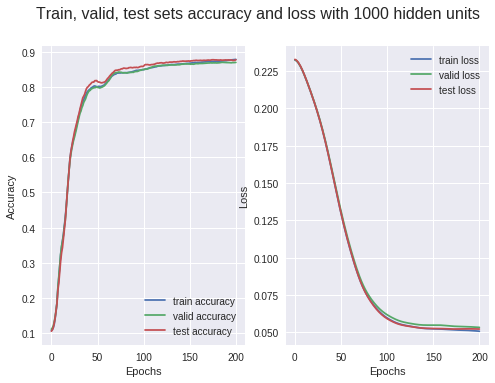
\includegraphics[width=.5\linewidth]{img/p1_3.png}
  \caption{Training, validation test set losses and accuracy.}
\end{figure}

In this task, we construct a neural network with hidden unit size of 1000. First, we initialize our weight matrices using the Xaiver initialization scheme. The hidden layer weight has zero-mean Gaussian distribution with variance of $\frac{1}{728+1000}$. And output layer weight has zero-mean Gaussian distribution with variance of $\frac{1}{1000+10}$. And bias matrices are assigned to zeros. Learning rate for this network is $0.0000001$, and $\gamma = 0.99$. The final accuracy we got are: 

\begin{table}[H]
\centering
{\small
\begin{tabular}{ccc}
\hline
 Training data accuracy  & Valid data accuracy      & Test data accuracy \\ \hline
88.06\% & 87.45\% & 88.18\% \\ \hline
\end{tabular}

}

\vspace{-0.2cm}
\caption{Training, validation and test accuracy after training.}
\label{tab:Learning}
\vspace{-0.4cm}

\end{table}

And this training took $323.45$ seconds. \\

\lstinputlisting[language=python, caption = Learning]{functions/learning.py}

\subsection{Hyper-parameter Investigation}

\subsubsection{Number of hidden units}

\begin{figure}[H]
\centering

  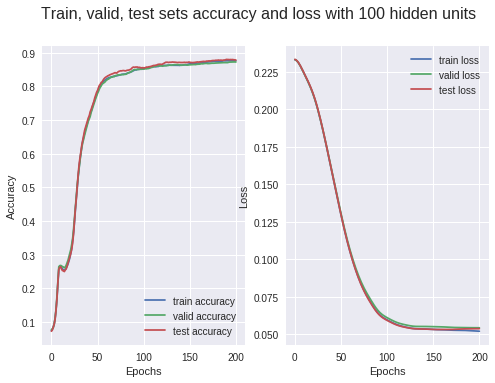
\includegraphics[width=.5\linewidth]{img/p1_4_1.png}\hfill
  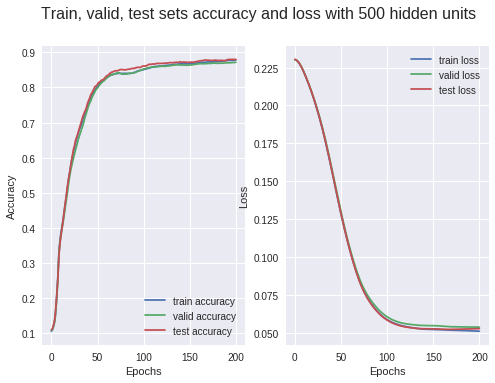
\includegraphics[width=.5\linewidth]{img/p1_4_2.png}\hfill
  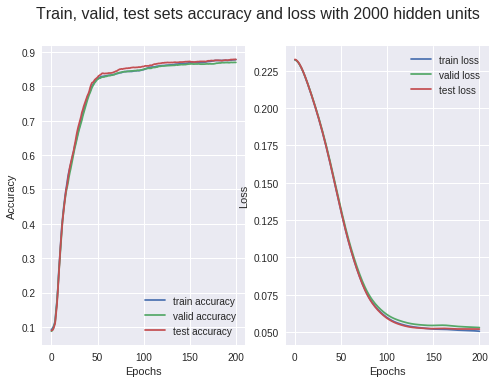
\includegraphics[width=.5\linewidth]{img/p1_4_3.png}
  \caption{Accuracy and losses with different hidden units.}

\end{figure}


\begin{table}[H]
\centering
{\small

\begin{tabular}{ccccc}
\hline
 & Training data accuracy  & Valid data accuracy      & Test data accuracy & Training time \\ \hline
Hidden units = 100 & 87.31\% & 87.01\% & 87.81\% & 39.75s\\ 
Hidden units = 500 & 87.85\% & 87.53\% & 88.21\% & 136.81s\\ 
Hidden units = 2000 & 88.14\% & 87.53\% & 88.21\% & 444.40s\\ \hline
\end{tabular}
}

\vspace{-0.2cm}
\caption{Training, validation and test accuracy after training.}
\label{tab:Number of hidden units}
\vspace{-0.4cm}
\end{table}

From table 2 above, we could see the accuracy for all three data sets have increased as the number of hidden units grow from 100 to 500. And from 500 to 2000, the time required for train the model was increasing largely, however, the accuracy for both validation data and test data remained the same, which means when the number of hidden units is around 500, the neural network obtained both high performance and high accuracy. One research suggested\cite{1189626} the optimal number of hidden units for first hidden layer can be calculated by $\sqrt{(m+2)N}+2\sqrt{N/(m+2)}$ , where N is the number of inputs, and m is the number of outputs, by using the formula, the optimal number of hidden units would be approximately 550 in this case, which is closer to 500 in table 2. 

\subsubsection{Early stopping}

The early stopping point could be found when the accuracy of the validation data reached its highest value\cite{Prechelt97earlystopping}. In the case of section 1.3, by training the model with 1000 hidden layers and 200 epochs, the highest accuracy for validation data occurred at the end of 200 epochs. The accuracy for each of three data sets are: 88.06\% for training data, 87.45\% for valid data, and 88.18\% for test data. There was no early stopping point for 200 epochs, and even when the epochs increased to 300, the over fitting still didn't occur. The highest accuracy for valid data is at the last iteration, which are: 89.01\% for training data, 88.28\% for valid data, and 88.66\% for test data. 



\section{Neural Networks in Tensorflow}



\subsection{Model implementation}

 For the neural network parameters, since the image is $28\times 28 = 728$ and single channel, we define a input placeholder $x$, which has shape of $[None, 28, 28, 1]$. Here the row dimension is "None", because that we need the network to dynamically adapt our batch size. This tells placeholder that they will receive this dimension at the time when we will feed in the data to them. Similarly, for output placeholder, it has shape of $[None, n\_classes]$. Here $\textit{n\_classes}   = 10$. \\

As for weights and biases, we initialize them with the Xavier scheme. The first convolution layer has $32-4\times4$ filters, so the first key "wc1" in the weight dictionary has a shape of $[3, 3, 1, 32]$. The first and second numbers are filter size, the third is the number of channels in the input image, which is $1$. And last represents the number of filters.  \\

After applying convolution and max pooling operations, we are down-sampling the input image from $28\times28\times1$ to $14\times14\times1$. And we need to flatten this down-sampled output to feed the fully connected layer. And we also decided to double the output size of this layer. Hence, weight "wc2" has a shape of $[14\times14\times32, 64]$. Similarly, second fully connected layer has a shape of $[64, 128]$. Finally, the output layer of this neural network should have dimension equals to previous layer output channels times the number of classes.  \\

Same principle for biases initialization.  

\lstinputlisting[language=python, caption = Weights and bias initialization]{functions/conv_nn_weights_bias_init.py}

Two functions below are convolution and max-pooling layers. And convolution layer has ReLU activation function. In the \textit{conv2d()} function we passed 4 arguments: input x, weights W, bias b and strides. This last argument is by requirement set to 1,

\lstinputlisting[language=python, caption = Convolutional layer functions ]{functions/conv_nn_util.py}

The \textit{conv\_net()} function takes 3 arguments as an input: the input x and the weights and biases dictionaries. This function build up the architecture of our convolutional neural network. Detailed layer interpretation is documented in the code below. \\

At this point, we can start with constructing the training model by call the \textit{conv\_net()} function. Since this is a multi-class classification problem, we are going to use softmax activation on the output layer as implemented in line $42$ of below code. 

\lstinputlisting[language=python, caption = Neural network architecture]{functions/conv_nn.py}

Finally, we can training and testing the model. Define a loop to run number of training iterations that we specified, in this case is 50 epochs. Right after that, we initiate a second for loop, which is for the number of batches. After each training iteration is completed, shuffle the training data. 

\lstinputlisting[language=python, caption = Train session]{functions/conv_nn_session.py}

\subsection{Model Training}
\begin{figure}[H]
\centering

  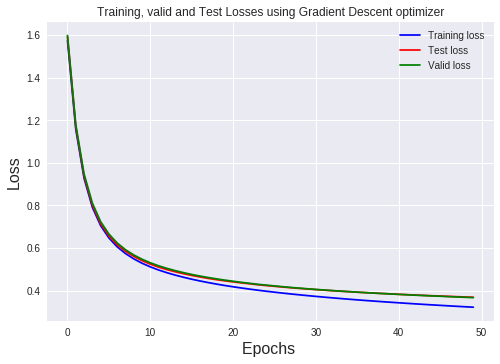
\includegraphics[width=.4\linewidth]{img/p2_2_SGD_loss.png}\hfill
  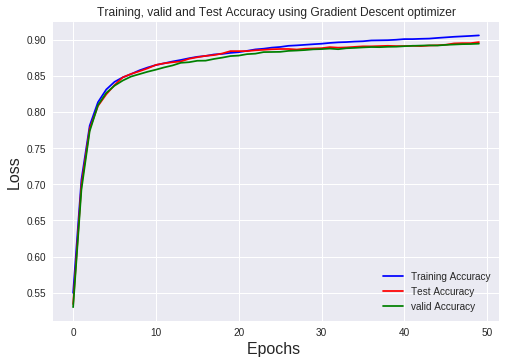
\includegraphics[width=.4\linewidth]{img/p2_2_SGD_acc.png}\hfill
  \caption{Accuracy and losses of CNN using SGD optimizer.}

\end{figure}

\begin{figure}[H]
\centering

  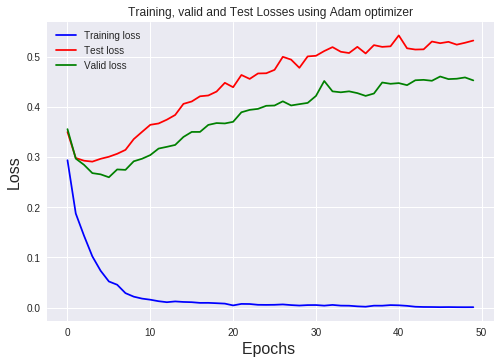
\includegraphics[width=.5\linewidth]{img/p2_2_adam_loss.png}\hfill
  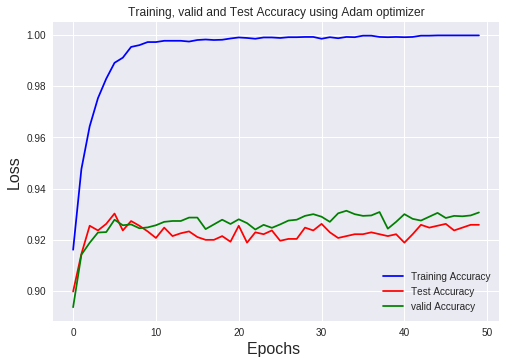
\includegraphics[width=.5\linewidth]{img/p2_2_adam_acc.png}\hfill
  \caption{Accuracy and losses of CNN using Adam optimizer.}

\end{figure}

\subsection{Hyper-parameter Investigation}

Notice that previous part, when we train the model using Adam Optimizer, a significant over-fitting occurred. But it is not the case for SGD. Therefore, we are not going to consider SGD in this part. 

\subsubsection{L2 Normalization}


\begin{table}[H]
\centering
% \tabcolsep=0.14cm
{\small
\begin{tabular}{rrrr}
\hline
      \lambda     &   Training Accuracy &   Validation Accuracy &   Testing Accuracy   \\
\hline
0     &     99.97\%  &      93.13\%  &      93.06\%  \\
0.01 &     99.61\% &      93.41\% &      92.58\% \\
0.1 &     93.12\% &      91.43\% &      91.59\% \\
0.5 &     87.58\% &      86.45\% &      87.37\% \\
\hline
\end{tabular}
}
\vspace{-0.2cm}
\caption{Final training, validation and test accuracy for different regularization}
\label{tab:L2 Normalization}
\vspace{-0.4cm}
\end{table}

\begin{figure}[H]
\centering
  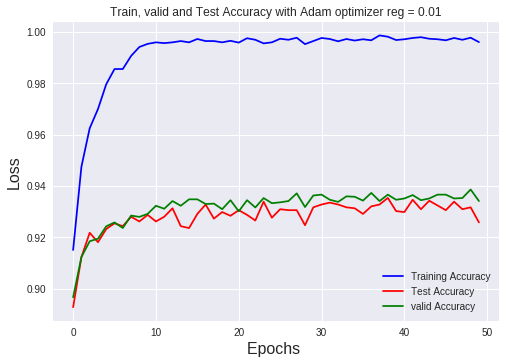
\includegraphics[width=.33\linewidth]{img/p2_3_adam_acc1.png}\hfill
  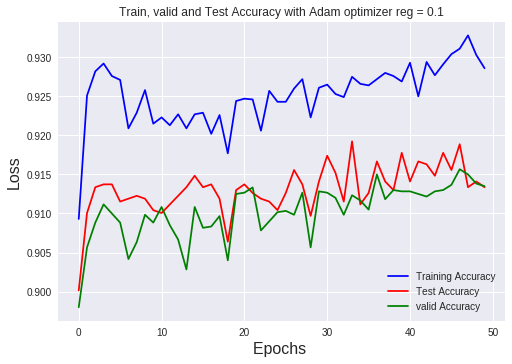
\includegraphics[width=.33\linewidth]{img/p2_3_adam_acc2.png}\hfill
  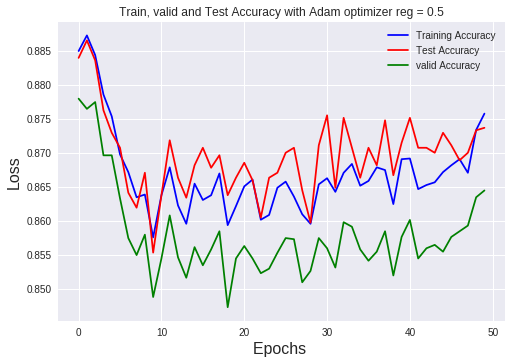
\includegraphics[width=.33\linewidth]{img/p2_3_adam_acc3.png}\hfill
  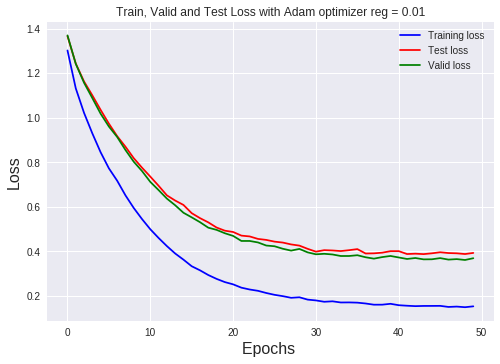
\includegraphics[width=.33\linewidth]{img/p2_3_adam_loss1.png}\hfill
  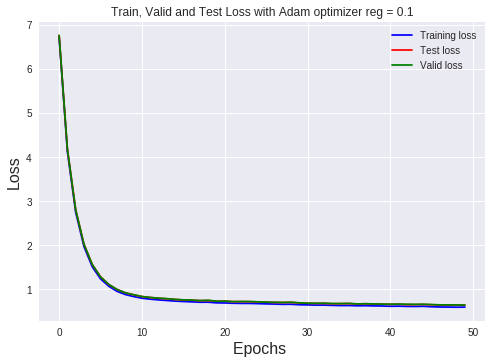
\includegraphics[width=.33\linewidth]{img/p2_3_adam_loss2.png}\hfill
  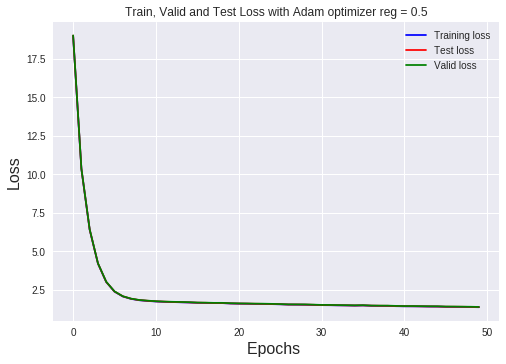
\includegraphics[width=.33\linewidth]{img/p2_3_adam_loss3.png}\hfill
  \caption{Training, validation and test accuracy and loss curves for different regularization.}
\end{figure}

Adding L2 regularization is one way to prevent the model from over fitting the training data, by changing the decay coefficient $\lambda$, the accuracy of the training model changes. As shown in table 3, as $\lambda$ increased, the accuracy of all three data sets decreased, since L2 used squares, it already had emphasized the error, and in addition, the $\lambda$ parameter which is directly proportional to the penalty is also stronger the penalty as the coefficient increased, therefore, as the penalty (decay coefficient) increased, there will be more noise added to the model, it did prevent the model from over fitting, however, it also leads to a lower accuracy. 


\subsubsection{Dropout}
\begin{table}[H]
\centering
% \tabcolsep=0.14cm
{\small
\begin{tabular}{rrrr}
\hline
      Deprecated &   Training Accuracy &   Validation Accuracy &   Testing Accuracy  \\
\hline
0     &     99.97\%  &      93.13\%  &      93.06\%  \\
0.9 &     99.82\% &      92.35\% &      92.62\% \\
0.75 &     99.43\% &      92.33\% &      92.03\% \\
0.5 &     98.56\% &      91.87\% &      91.63\% \\
\hline
\end{tabular}
}
\vspace{-0.2cm}
\caption{Final training, validation and test accuracy for different dropout rates}
\label{tab:Dropou}
\vspace{-0.4cm}
\end{table}

\begin{figure}[H]
\centering
  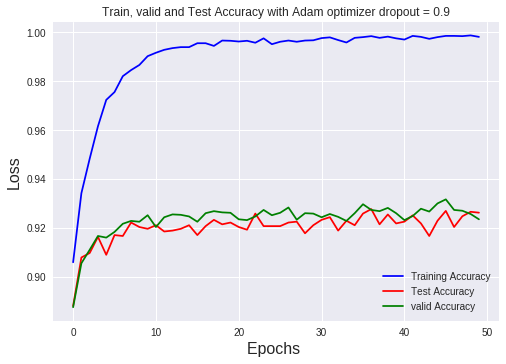
\includegraphics[width=.33\linewidth]{img/p2_3_adam_acc1_1.png}\hfill
  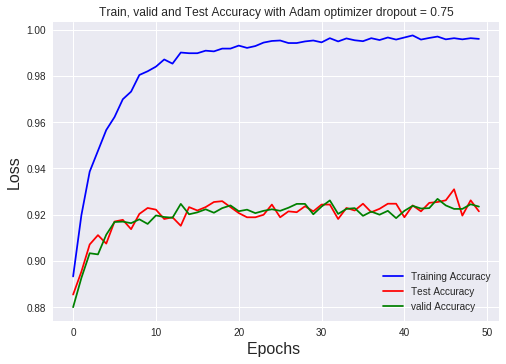
\includegraphics[width=.33\linewidth]{img/p2_3_adam_acc2_2.png}\hfill
  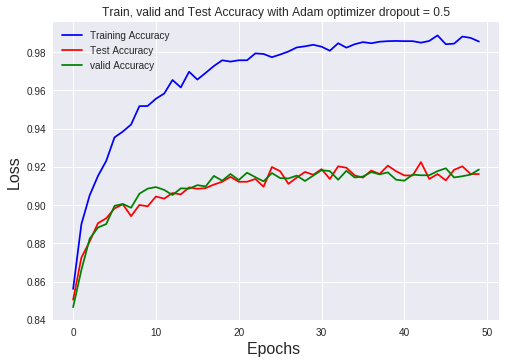
\includegraphics[width=.33\linewidth]{img/p2_3_adam_acc3_3.png}\hfill
  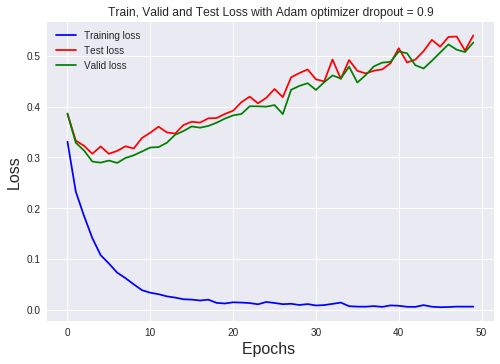
\includegraphics[width=.33\linewidth]{img/p2_3_adam_loss1_1.png}\hfill
  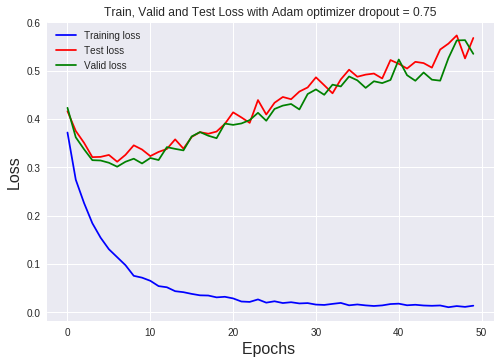
\includegraphics[width=.33\linewidth]{img/p2_3_adam_loss2_2.png}\hfill
  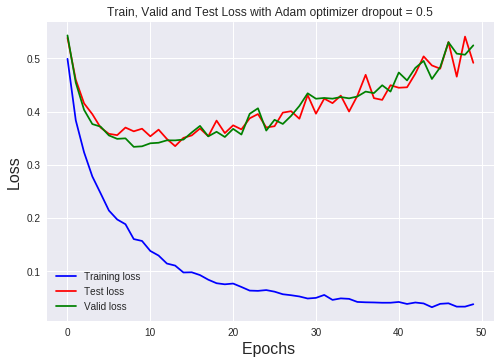
\includegraphics[width=.33\linewidth]{img/p2_3_adam_loss3_3.png}\hfill
  \caption{Training, validation and test accuracy and loss curves for different regularization.}
\end{figure}
Another way to control model from over fitting is to add dropouts to certain layers. As shown in table 4 above, the "Deprecated" column had shown the probability of each hidden unit that will not be dropped out, such as 0.9 means there are a 10\% chance for each hidden unit to be set to 0 (drop out). As the probability of dropout unit increased, more noise were added to the training model, therefore, the accuracy for all three data sets had decreased. \\



\\
\medskip
\vspace{15mm}

\bibliographystyle{ieeetr}
\bibliography{earlystopping}




\end{document}
